\documentclass[aspectratio=169]{beamer}

\usepackage[utf8]{inputenc}
\usepackage[english]{babel}
\usepackage[T1]{fontenc}
\usepackage{lmodern}
\usepackage{bbm}
\usepackage{listings}
\usepackage{multicol}
\usepackage{csquotes}
\usepackage{hyperref}
\usepackage{indentfirst}
\usepackage{amsthm}
\usepackage{amsfonts}
\usepackage{amsmath}
\usepackage{amssymb}
\usepackage{mathtools}
\usepackage{tikz}
\usepackage{xcolor}
\usepackage{array}
\usepackage{bookmark}
\usepackage{booktabs}

\newcommand{\id}[1]{\ensuremath{\mathit{#1}}}
\newcommand{\kw}[1]{\ensuremath{\mathtt{#1}}}
\newcommand{\Let}{\kw{let}}
\newcommand{\In}{\kw{in}}
\newcommand{\If}{\kw{if}}
\newcommand{\Then}{\kw{then}}
\newcommand{\Else}{\kw{else}}
\newcommand{\Filter}{\kw{filter}}
\newcommand{\Or}{\kw{or}}
\newcommand{\Groupby}{\kw{groupby}}
\newcommand{\Partition}{\kw{partition}}
\newcommand{\Scatter}{\kw{scatter}}
\newcommand{\Hist}{\kw{hist}}
\newcommand{\Map}{\kw{map}}
\newcommand{\Sum}{\kw{sum}}
\newcommand{\Mod}{\kw{mod}}
\newcommand{\Fst}{\kw{fst}}
\newcommand{\Snd}{\kw{snd}}
\newcommand{\Presum}{\kw{presum}}
\newcommand{\True}{\kw{true}}
\newcommand{\False}{\kw{false}}
\newcommand{\Sort}{\kw{sort}}
\newcommand{\Segor}{\kw{segor}}
\newcommand{\Hash}{\kw{hash}}
\newcommand{\Random}{\kw{random}}
\newcommand{\Iota}{\kw{iota}}
\newcommand{\Unzip}{\kw{unzip}}
\newcommand{\Unit}{\mathbf{unit}}
\newcommand{\Int}{\mathbf{int}}
\newcommand{\Bool}{\mathbf{bool}}
\newcommand{\Def}{\kw{def}}
\newcommand{\While}{\kw{while}}
\newcommand{\Do}{\kw{do}}
\newcommand{\Rep}{\kw{rep}}
\newcommand{\Zip}{\kw{zip}}

\usetikzlibrary{automata, positioning, arrows}

\graphicspath{ {./figures/} }

\definecolor{palepurple}{rgb}{0.7647,0.69411,0.88235}
\definecolor{palepurple}{rgb}{0.7647,0.69411,0.88235}
\definecolor{midviolet}{rgb}{0.6,0.4,0.8}

\newcolumntype{M}[2]{>{\centering\arraybackslash}m{#1}<{\rule{0pt}{#2}}}
\newcommand{\darkpalepurple}{palepurple!70!black}
\definecolor{paleyellow}{rgb}{1.0,1.0,0.7725}
\setbeamercolor{background canvas}{bg=paleyellow}

\usetheme{default}
\usecolortheme{wolverine}
\setbeamercolor*{palette primary}{bg=palepurple}
\setbeamercolor*{palette quaternary}{bg=palepurple}
\setbeamercolor{structure}{fg=palepurple}
\setbeamertemplate{navigation symbols}{\insertframenumber/\inserttotalframenumber}
\setbeamertemplate{blocks}[rounded][shadow]
\setbeamercolor{frametitle}{bg=midviolet,fg=black}
\setbeamercolor{block title}{bg=structure, fg=black}
\setbeamercolor{block body}{bg=structure, fg=black}
\setbeamercolor{block title alerted}{bg=structure, fg=black}
\setbeamercolor{block body alerted}{bg=structure, fg=black}
\setbeamercolor{block title example}{bg=structure, fg=black}
\setbeamercolor{block body example}{bg=structure, fg=black}
\setbeamercolor{frametitle}{bg=palepurple,fg=black}


\setbeamertemplate{itemize item}{\scriptsize$\blacksquare$}
\setbeamertemplate{itemize subitem}{\scriptsize$\blacksquare$}
\setbeamertemplate{itemize subsubitem}{\scriptsize$\blacksquare$}

\title[Hash Maps]{Regular Expressions}
\author{\textbf{William Henrich Due} \inst{1}}
\institute[shortinst]{\inst{1} Department of Computer Science}
\date{September 12th, 2025}

\begin{document}

\begin{frame}
  \begin{center}
    \titlepage
    \vfill
  \end{center}
\end{frame}

\begin{frame}\frametitle{Intended Learning Outcomes}
  \begin{itemize}
    \item Come up with compilation rules from Regular Expressions to NFAs.
  \end{itemize}
\end{frame}

\begin{frame}\frametitle{Languages}
  \begin{itemize}
    \item Formal languages: Languages that have a formal definition.
    \item What Formal Languages do you know?
  \end{itemize}
\end{frame}

\begin{frame}\frametitle{Define Regular Expressions}
  
  \begin{itemize}
    \item Empty string: $\epsilon$
    \item Some letter: $\alpha$
    \item Some expression: $\mathcal{R}$
    \item Concatenation: $\mathcal{R}_0\mathcal{R}_1$
    \item Pattern to find: $sos$
    
    \vspace{10pt}
    \textbf{Inputs}
    \begin{itemize}
      \item No match: ${\color{red} something}$
      \item A match: $ab{\color{green}}$
    \end{itemize}
  \end{itemize}
\end{frame}

\begin{frame}\frametitle{Compilation}
  
\begin{align*}
  \mathcal{C}(s, s', \epsilon) \mapsto &
  \vcenter{
    \hbox{
      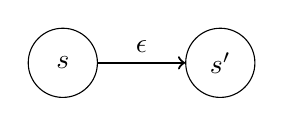
\begin{tikzpicture}[node distance=2cm, baseline]
        \node[state] (s) at (0,0) {$s$};
        \node[state] (sp) at (2,0) {$s'$};
        \draw[->, thick] (s) -- node[above] {$\epsilon$} (sp);
      \end{tikzpicture}
    }
  } \\
  \mathcal{C}(s, s', \alpha) \mapsto &
  \vcenter{
    \hbox{
      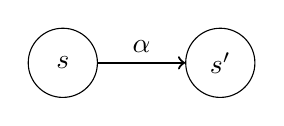
\begin{tikzpicture}[node distance=2cm, baseline]
        \node[state] (s) at (0,0) {$s$};
        \node[state] (sp) at (2,0) {$s'$};
        \draw[->, thick] (s) -- node[above] {$\alpha$} (sp);
      \end{tikzpicture}
    }
  }\\
  \mathcal{C}(s, s', \mathcal{R}_0\mathcal{R}_1) \mapsto &
  \vcenter{
    \hbox{
      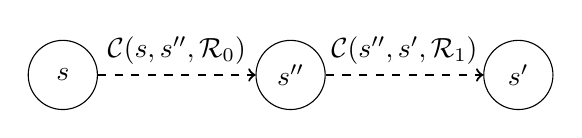
\begin{tikzpicture}[node distance=2cm, baseline]
        \node[state] (s) {$s$};
        \node[state] (si) [right=of s] {$s''$};
        \node[state] (sp) [right=of si] {$s'$};
        \draw[->, dashed, thick] (s) -- node[above] {$\mathcal{C}(s, s'', \mathcal{R}_0)$} (si);
        \draw[->, dashed, thick] (si) -- node[above] {$\mathcal{C}(s'', s', \mathcal{R}_1)$} (sp);
      \end{tikzpicture}
    }
  }
\end{align*}
\end{frame}
\end{document}